\documentclass{article}
\usepackage[utf8]{inputenc}
\usepackage[T1]{fontenc} 
\usepackage[polish]{babel}
\usepackage{enumitem}
\usepackage{graphicx}
\usepackage[table]{xcolor}

\title{Raport 1. \\ \large Zmiany w demografii w Polsce w latach 2002 oraz 2022}
\author{Kacper Ujma \and Michał Strugacz}
\date{06.05.2024}

\addto\captionspolish{%
	\renewcommand{\bibname}{Literatura}
}

\begin{document}
	\maketitle
	
	\begin{enumerate}
		\item \textbf{Wstęp}\\
		Demografia rozwiniętych państw europejskich zmieniła się znacząco na przestrzeni lat. Aby to pokazać, użyjemy danych struktury ludności w Polsce na przestrzeni 20 lat, konkretnie w latach 2002\cite{bib2002} oraz 2022\cite{bib2023}. Skupimy się na rozkładzie ludności w różnych przedziałach wiekowych. W tym celu użyjemy podstawowych zmiennych statystycznych, takich jak średnia arytmetyczna itp. Przeanalizujemy dane z wykorzystaniem programów napisanych w języku Python, za pomocą których zilustrujemy również zmiany w polskim społeczeństwie.
		
		
		\item \textbf{Analiza danych demograficznych}
		
		\begin{enumerate}[label*=\arabic*.]
			\item \textbf{Wstęp}\\
			W celu analizy danych użyjemy pewnego uproszczenia. Ponieważ w zbiorach danych osoby w wieku powyżej stu lat zostały zsumowane do jednej grupy, w analizie zbioru ludzi z tej grupy potraktujemy jako 100-letnich.
			
			\item \textbf{Przedstawienie danych}\\
			Dane na temat ilości ludzi w różnym wieku przedstawimy za pomocą dwóch histogramów. Będą one kluczowe do zrozumienia dalszych rozważań na temat struktury społeczeństwa, ponieważ ilustrują wszystko, o czym później będzie mowa.
			
			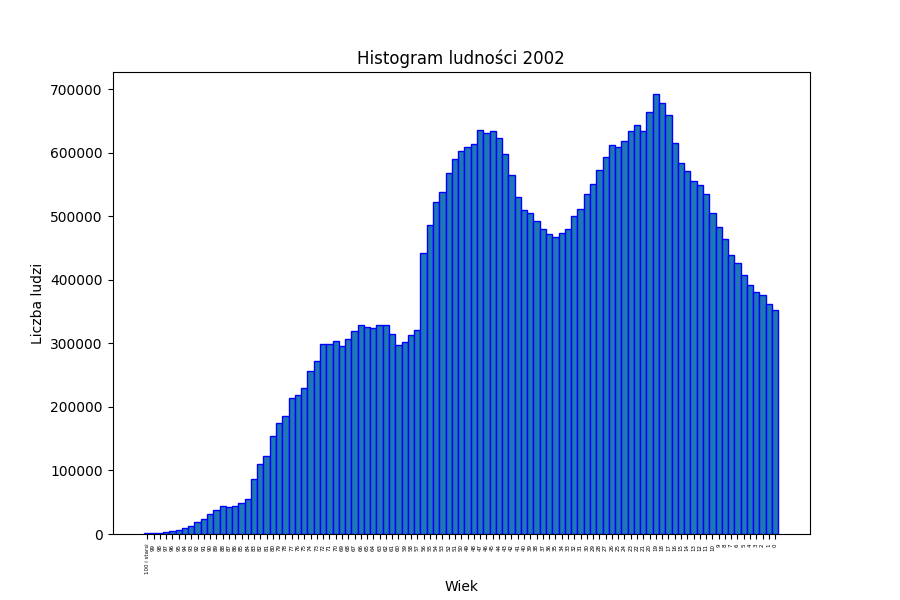
\includegraphics[scale=0.4]{"C:/Users/kacpu/Programowanie/Semestr4/Statystyka stosowana/Raport1/Wykresy/Histogram_2002.png"}
			
			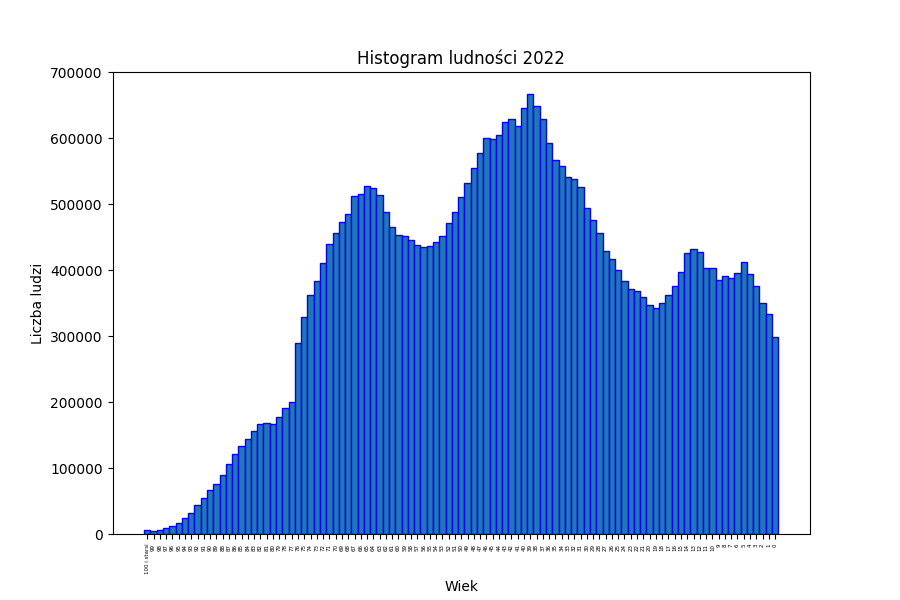
\includegraphics[scale=0.4]{"C:/Users/kacpu/Programowanie/Semestr4/Statystyka stosowana/Raport1/Wykresy/Histogram_2022.png"}
			
			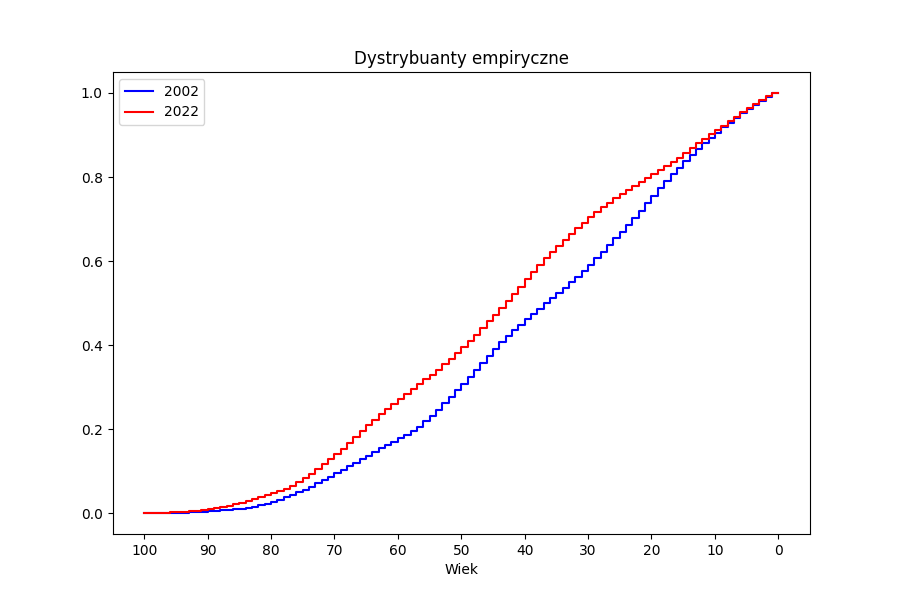
\includegraphics[scale=0.4]{"C:/Users/kacpu/Programowanie/Semestr4/Statystyka stosowana/Raport1/Wykresy/Dystrybuanty_empiryczne.png"}
			
			Pierwszy histogram posiada dwie "górki" ludzi w wieku około 46 i 19 lat. Zauważamy także znaczący spadek liczby ludzi starszych niż 57 lat oraz spadek urodzeń od rocznika 1990.
			
			Na histogramie z 2022 roku widzimy te same "górki" co wcześniej, lecz przesunięte o 20 lat oraz pomniejszone o liczbę zgonów. Dodatkowo zauważamy wzrost liczby urodzeń ludzi od roku 2003, który okazuje się być pierwszym najmniejszym rocznikiem względem ilości urodzeń, aż do roku 2021, gdzie ilość ta jest rekordowa i dalej maleje.
			
			Porównując histogramy, możemy zauważyć pierwsze różnice i podobieństwa. Najważniejszą zauważalną różnicą jest przede wszystkim zmniejszenie się liczby ludności w młodym wieku do lat 20. Liczba urodzeń znacznie spada od 1990 roku, a kolejne urodzenia po znaczącym spadku nie równoważą postarzałych ludzi w ciągu 20 lat. Większość społeczeństwa przesuwa się w lewą stronę, to znaczy większą część społeczeństwa stanowią ludzie starsi niż w 2002 roku, co ma odzwierciedlenie w zmiennych statystycznych.
			
			Ta sama tendencja uwidacznia się na wykresie dystrybuant. Znacznie szybszy wzrost dystrybuanty z 2022 pokrywa się z cięższym ogonem z lewej strony natomiast najszybszy wzrost dla 2002 roku zauważalny jest dopiero przy młodszym wieku.
			
			
			
			\item \textbf{Średnie}\\
			Pierwszą średnią, którą policzymy, będzie oczywiście średnia arytmetyczna, wynosząca dla danych z 2002 roku około 37 lat, a dla 2022 roku około 42 lat. Różnica wynosi aż 5 lat. Tak znacząca różnica jest widoczna na histogramach oraz pokrywa się z wyciągniętymi wnioskami.
			
			Dalsze rozważania kontynuujemy, licząc średnie cięte obu społeczeństw.
			
			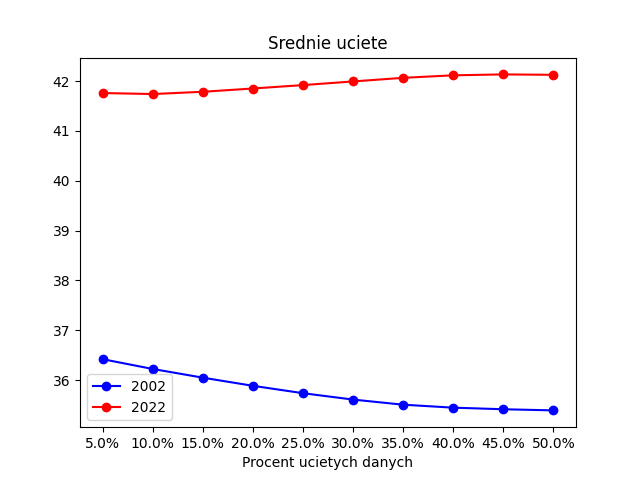
\includegraphics[scale=0.5]{"C:/Users/kacpu/Programowanie/Semestr4/Statystyka stosowana/Raport1/Wykresy/Srednie_ciete.png"}
			
			Zachowanie średnich jest odmienne. Dla 2002 roku zauważamy trend spadkowy, co sugeruje nam spory udział młodej grupy w społeczeństwie, gdyż przedział wiekowy tej grupy jest mniejszy od grupy starszych. Z kolei niewiele rosnąca średnia z 2022 roku wskazuje na większą ilość ludzi w wieku średnim oraz starczym.
			
			Średnie harmonicze to kolejne narzędzie do analizy otrzymanych wyników. Wynoszą one odpowiednio dla 2002 roku 17,1 oraz dla 2022 roku 18,9. Wzrost średniej na przestrzeni 20 lat wskazuje na zwiększenie udziału starszych w społeczeństwie oraz na mniej równomierny rozkład społeczeństwa.
			
			\item \textbf{Kwantyle}\\
			
			\begin{table}[h]
				\centering
				\label{tab:przyklad_linie}
				\begin{tabular}{|c|c|c|}
					\hline
					Kwantyle & 2002 & 2022 \\
					\hline
					Pierwszy & 19 & 24 \\
					\hline
					Drugi & 35 & 42 \\
					\hline
					Trzeci & 52 & 60 \\
					\hline
				\end{tabular}
			\end{table}
			
			Z tabeli wyciągamy wnioski, iż w społeczeństwie 2002 roku przeważającą część społeczeństwa stanowią ludzie młodzi. Aż połowa społeczeństwa mieści się w małej części przedziału wiekowego (35\%). Sytuacja w 2022 roku jest odmienna, większość społeczeństwa starzeje się. Widoczna różnica, natomiast nie stosuje się do rozstępu międzykwantylowego. W 2002 wynosił 33 lata, a w 2022 tylko 36. Wynika z tego, że połowa ludzi mieści się w zakresie szerszym tylko o 3 lata. Taki wynik jest spowodowany przesunięciem się (postarzeniem) dominujących grup wiekowych w 2002 roku i brakiem wystarczająco dużego młodego pokolenia przez ten czas, które utrzymałoby ciężar społeczeństwa na młodych.
			
			\item \textbf{Wariancja i odchylenie standardowe}\\
			
			\begin{table}[h]
				\centering
				\begin{tabular}{|c|c|c|}
					\hline
					\cellcolor{gray!40} & 2002 & 2022 \\
					\hline
					Wariancja & 467,1 & 516,2 \\
					\hline
					Odchylenie standardowe & 21,6 & 22,7 \\
					\hline
				\end{tabular}
			\end{table}            
			
			Na przestrzeni 20 lat odchylenie standardowe rośnie, z czego wynika wzrost rozproszenia w społeczeństwie. Mając na uwadze poprzednie wnioski, zauważamy większe znaczenia starszych w społeczeństwie. Kolejnym zauważonym faktem jest to, że odchylenie jest większe niż połowa rozstępu międzykwantylowego. Wskazuje to na brak skupienia społeczeństwa wokół średniej arytmetycznej. Społeczeństwo nie jest jednorodne i znajdują się w nim duże grupy oddalone od średniej. Nierówność ta na przestrzeni czasu zmniejsza się, co świadczy o zagęszczeniu się danych. W kontekście demografii znaczy to, że liczba urodzeń maleje.
			
			
			\item \textbf{Kurtoza i skośność}\\
			\begin{table}[htpb]
				\centering
				\begin{tabular}{|c|c|c|}
					\hline
					\cellcolor{gray!40}    & 2002 & 2022 \\
					\hline
					Kurtoza & -0,819 & -0,887 \\
					\hline
					Skośność & -0,2780 & -0,0155 \\
					\hline
				\end{tabular}
			\end{table}
			
			Patrząc na histogramy społeczeństw, można łatwo określić ich kształt, jednak zauważone różnice objawiają się w policzonych kurtozach i skośnościach.

			Kurtoza rozkładu zmniejsza się niewiele, sugerując nam zmniejszenie się znaczenia skrajnych danych rozkładu społeczeństwa. Po raz kolejny potwierdza nam to przeniesienie się średniej rozkładu demograficznego do centrum wieku na skali od 0 do 100. Różnica w skośności jest natomiast bardzo znacząca. Zauważamy skłonność danych do symetryczności. Ze społeczeństwa o dużym znaczeniu młodego wieku koncentruje się wokół coraz większej średniej wieku. Ta zmiana mówi nam najwięcej o tendencji zmian w demografii.  
			
		\end{enumerate}
		
		\item \textbf{Wnioski}\\
		Najważniejszym wnioskiem wyciągniętym z analizy danych demograficznych z lat 2002 oraz 2022 jest starzenie się społeczeństwa. Zwizualizowany na boxplotach.
		
		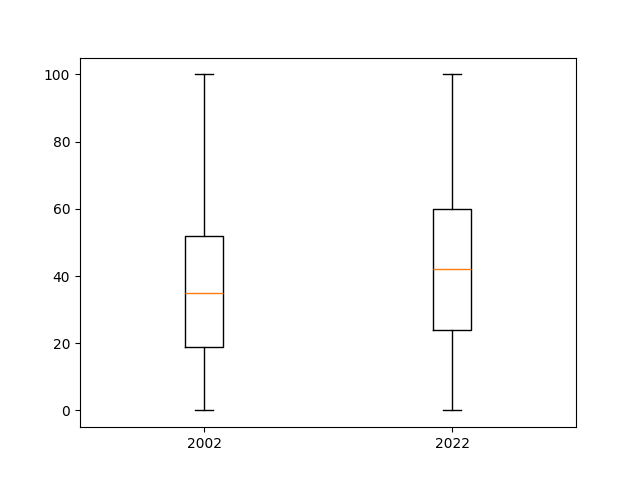
\includegraphics[scale=0.5]{"C:/Users/kacpu/Programowanie/Semestr4/Statystyka stosowana/Raport1/Wykresy/Boxploty.png"}
		
		Widoczne na wykresie przesunięcie pudełka ku górze jest znaczące biorąc pod uwagę równicę zaledwie 20 lat.
		Trend ten jest jednoznaczny i widoczny w analizach danych. Średni wiek Polaków w 2022 roku był o 5 lat wyższy niż w 2002 roku. To oznacza, że społeczeństwo polskie staje się coraz starsze. 
		Wyliczone kwantyle bezsprzecznie wskazują na przenoszenie się ciężaru społeczeństwa na jego starszą część oraz na zmniejszenie się liczby urodzeń. Kolejno zauważamy nierównomierne rozłożenie wieku. Spadki liczby urodzen w latach 90 oraz 2010 prowadzą do nierównomiernej dystrybucji, lecz z tendencją do zagęszczania się danych wokół coraz większej średniej. Analiza kurtozy i skośności rozkładu wieku wskazuje na zmniejszenie się znaczenia skrajnych danych. To sugeruje, że społeczeństwo, które kiedyś charakteryzowało się dużym odsetkiem młodych ludzi, teraz przesuwa się ku coraz starszym grupom wiekowym.
		
	\end{enumerate}
	
	\begin{thebibliography}{9}
		\bibitem{bib2002} 
		Dane demograficzne Polski w roku 2002 według płci i wieku: [https://demografia.stat.gov.pl/bazademografia/Tables.aspx].
		
		\bibitem{bib2023} 
		Dane demograficzne Polski w roku 2023 według płci i wieku: [https://demografia.stat.gov.pl/bazademografia/Tables.aspx].
	\end{thebibliography}
	
\end{document}
